% (15-25)
%
% DESIGN DE SOFTWARE
% DEFINIR REDE DE SOFTWARE
% CLUSTERING
% AVALIAÇÃO DE CLUSTERING
% 
%     * redes complexas
%     * designs de software como redes complexas
%     * conceito de tríadas como base para caracterização de redes complexas
%     * clustering
%     * avaliação de algoritmos de clustering

\chapter{Agrupamento de Software} \label{cap:agrupamento}

% TODO: Onde falar sobre extração do design?

\begin{section}{Recuperação de Arquitetura de Software}

A arquitetura de um sistema de software é formada pelas decisões mais significativas sobre o desenvolvimento do sistema [Booch, 2006]. Essas decisões devem ser tomadas preferencialmente nos estágios iniciais do processo de desenvolvimento, pois elas afetam um grande número de decisões ao longo do ciclo de vida do software.

É comum documentar uma arquitetura como um conjunto de visões, na qual cada visão descreve decisões que dizem respeito a um subconjunto dos requisitos do sistema \cite{Clements2002}. A visão modular é a mais importante no gerenciamento da evolução de software \cite{Parnas1972}. Ela representa a organização de um sistema em módulos com responsabilidades bem definidas e descreve interações entre os módulos. A visão modular facilita a análise de atributos como facilidade de modificação e possibilidade de reuso de partes do sistema.

Muitos sistemas, no entanto, não possuem uma arquitetura bem documentada. Durante o desenvolvimento de um sistema, a documentação de sua arquitetura pode tornar-se desatualizada, resultando em uma deterioração da estrutura do sistema \cite{Eick2001,Parnas1994}. O problema se agrava quando os desenvolvedores originais abandonam o projeto, levando com eles um conhecimento tácito sobre a arquitetura do sistema.

O termo recuperação de arquitetura (ou reconstrução de arquitetura) se refere a métodos que extraem aspectos da arquitetura de um sistema a partir de artefatos criados durante seu desenvolvimento, como o código-fonte \cite{Pollet2007}. Tais métodos têm sido usados como auxílio em tarefas como a documentação da arquitetura e a compreensão de sistemas legados \cite{Wu2005}.

Uma abordagem bastante pesquisada para auxiliar a compreensão e a documentação da visão modular da arquitetura de sistemas é chamada agrupamento de software \cite{Mancoridis1998,Andritsos2005,Maqbool2007}. Algoritmos de agrupamento de software agrupam o conjunto de entidades do código-fonte de um sistema (por exemplo, classes em um sistema orientado a objetos) em subconjuntos denominados módulos. O agrupamento é feito de forma que, sob algum critério, as entidades agrupadas em um mesmo módulo possuem grande similaridade entre si e pequena similaridade com entidades que estão em outros módulos. Vale ressaltar que o termo agrupamento designa tanto a atividade de agrupamento como o resultado dessa atividade, que é a organização das entidades analisadas em módulos.

Naturalmente, o problema de agrupar entidades segundo algum critério de similaridade não é exclusivo do domínio de software. O problema tem sido objeto da mineração de dados, da inteligência artificial, do estudo de redes sociais etc. Assim como em outros domínios, o problema de agrupamento de software não é bem definido no domínio de recuperação de arquitetura. A definição de qual é o melhor agrupamento é subjetiva. Ainda assim, o agrupamento dos dados pode evidenciar relacionamentos existentes entre entidades e servir como ponto de partida de atividades como, por exemplo, a atribuição de arquivos de código-fonte a programadores.

% Falar sobre escolha das entidades e da descrição das entidades (citar Anquetil antigo, que usa nome de arquivo, e Anquetil novo, que compara resultados de diversas descrições, e Kuhn2005). AQUI? Onde?

\end{section}

\begin{section}{Algoritmos de Agrupamento de Software}

Para realizar o agrupamento automático de um conjunto de entidades, as seguintes questões devem ser consideradas:

\begin{itemize}
	\item a identificação das entidades;
	\item a descrição das entidades;
	\item o algoritmo de agrupamento;
\end{itemize}

No domínio do agrupamento de software, exemplos de entidades incluem, entre outros, arquivos fonte \cite{Mancoridis1998}, funções e variáveis em um sistema procedimental \cite{Anquetil1999} e classes em um sistema orientado a objetos \cite{Trifu2001}.

A descrição das entidades determina as características a se considerar para determinar se duas entidades são mais ou menos similares. Por exemplo, se o objetivo é agrupar classes em um programa orientado a objetos, as seguintes descrições, entre outras, podem ser adotadas para cada entidade:
%funções em um programa procedimental, as seguintes descrições, entre outras, podem ser adotadas para cada entidade:

\begin{itemize}
	% \item conjunto das palavras usadas nos comentários que descrevem a função;
	% \item conjunto dos programadores que trabalharam na função;
	\item conjunto das classes que especializam a classe descrita através do mecanismo de herança;
	\item conjunto das classes que definem métodos chamados pela classe descrita.
	% \item conjunto das funções chamadas pela função;
	% \item conjunto das variáveis manipuladas na função.
\end{itemize}

As descrições exemplificadas são chamadas de descrições formais, pois elas têm impacto sobre o comportamento do programa. Em muitos casos, as descrições formais de um sistema são representadas como um grafo, que é extraído a partir do código-fonte através da análise estática de seu código-fonte, uma abordagem que prescinde da execução do sistema.
% , e são as descrições mais estudadas no contexto de agrupamento de software \cite{Anquetil1999}

Algumas interações entre entidades de um sistema só se manifestam durante a execução do sistema e, por isso, não são identificadas em uma análise estática. Exemplos incluem a instanciação de objetos através de introspecção e a interação entre objetos que se comunicam através de um protocolo de troca de mensagens entre processos. Tais interações só podem ser identificadas através de uma análise dinâmica, que envolve a execução do sistema.

As relações entre entidades que podem ser identificadas através de análise estática são chamadas de dependências estáticas. Em um programa orientado a objetos, dependências estáticas entre classes incluem interações como a chamada de um método, a leitura ou escrita de um atributo, a instanciação de um objeto e a herança.

Neste trabalho, optou-se por estudar o agrupamento de software no caso em que o software é representado como um grafo de dependências estáticas entre entidades do código-fonte. Tal escolha se justifica pelo grande número de trabalhos que seguem essa abordagem. Em particular, neste trabalho serão estudados sistemas escritos em Java, uma linguagem orientada a objetos popular, para a qual existem diversas ferramentas disponíveis para análise estática.

% As duas primeiras descrições são ditas não-formais. 
% 
% Em muitos estudos, as descrições formais das entidades de um sistema são extraídas através de análise estática do código-fonte, isto é, uma análise que prescinde da execução do sistema.

% A descrição usada neste trabalho é o grafo de dependências estáticas entre classes de sistemas orientados a objetos. % XXX

% XXX
% Após a identificação das entidades a serem agrupadas, portanto, o processo de agrupamento é realizado em duas etapas: a extração das descrições das entidades e o agrupamento propriamente dito. A Figura XXX ilustra o processo, considerando uma descrição sob a forma de grafo.
% 
% \begin{figure}[htbp]
% 	\centering
% 		\includegraphics[scale=1]{file}
% 	\caption{caption}
% 	\label{fig:label}
% \end{figure}

A seguir são descritos brevemente alguns algoritmos de agrupamento de software que operam sobre grafos de dependências entre entidades. Para esta pesquisa foram escolhidos algoritmos estudados por diferentes grupos de pesquisa e com implementações disponíveis publicamente.

\begin{subsection}{Algoritmos Hierárquicos Aglomerativos}

Algoritmos hierárquicos aglomerativos têm sido aplicados a diversos problemas, incluindo o agrupamento de software \cite{Anquetil1999,Maqbool2007}. Essa família de algoritmos funciona com qualquer descrição de entidade, desde que seja fornecida uma métrica de similaridade entre pares de entidades. A similaridade entre duas entidades é medida em uma escala contínua de 0 a 1. O algoritmo é simples: inicia-se com um módulo para cada entidade e então mesclam-se sucessivamente os dois módulos mais similares até restar apenas um módulo com todas as entidades.

No contexto de recuperação de arquitetura de software, é comum descrever as entidades de código-fonte como um grafo de dependências entre entidades e usar a métrica de Jaccard para medir a similaridade entre duas entidades \cite{Anquetil1999}. Sejam X e Y duas entidades, e seja d(A) o conjunto de entidades ligadas à entidade A no grafo de dependências. A similaridade entre X e Y é dada pela expressão a seguir:

$$
\mathrm{sim}(X, Y) ~=~ \frac{|\mathrm{d}(X) \cap \mathrm{d}(Y)|}{|\mathrm{d}(X) \cup \mathrm{d}(Y)|}
$$

O que diferencia os algoritmos hierárquicos aglomerativos entre si é o critério usado para medir a similaridade entre dois módulos. Os dois critérios mais estudados no contexto de agrupamento são chamados de ligação simples (SL, do inglês \emph{single linkage}) e ligação completa (CL, do inglês \emph{complete linkage}). Na ligação simples, a similaridade entre dois módulos é computada como a maior similaridade entre pares de entidades tiradas uma de cada módulo. Na ligação completa é considerada a menor similaridade.

Naturalmente, um agrupamento que consiste de apenas um módulo com todas as entidades analisadas é de pouco valor. Por essa razão deve existir um critério de parada que interrompa o algoritmo antes de todos os módulos terem sido mesclados em um grande módulo. No contexto de agrupamento de software, o critério mais comumente usado é a altura de corte, $h$, que varia entre 0 e 1. Sob esse critério, o algoritmo interrompe sua execução quando a maior similaridade entre dois módulos é igual a $1 - h$. Assim, quanto maior a altura de corte $h$, menor o número de módulos do agrupamento resultante.
	
\end{subsection}

%%%%%%%%%

\begin{subsection}{Bunch}

Com a finalidade de auxiliar a compreensão de programas, o algoritmo Bunch \cite{Mancoridis1998} agrupa o conjunto de entidades de um programa de acordo com os relacionamentos existentes entre elas, representados como um grafo orientado. O agrupamento é tratado como um problema de otimização no qual o objetivo é maximizar uma função denominada qualidade de modularização (QM), que recompensa agrupamentos com muitas arestas internas (que ligam entidades de um mesmo módulo) e poucas arestas externas (que ligam entidades de módulos distintos).

% TODO: fórmula da QM

Encontrar um agrupamento que possui QM ótima é um problema intratável; por isso o algoritmo Bunch usa heurísticas como algoritmos genéticos e \emph{hill-climbing} para obter resultados quase ótimos.

\end{subsection}

%%%%%%%%%%

\begin{subsection}{ACDC}

O algoritmo ACDC \cite{Tzerpos2000} foi projetado com o intuito de encontrar agrupamentos que facilitam a compreensão de programas. Assim como o Bunch, ele opera sobre grafos orientados. Sua principal característica é a identificação de conjuntos dominantes de vértices no grafo. Um conjunto dominante é um conjunto de vértices, $v_0, v_1, \ldots{}, v_n$, onde $v_0$ é o vértice dominante, que satisfaz a duas condições: (i) existe um caminho entre $v_0$ e qualquer $v_i$; (ii) qualquer caminho de um vértice que não pertence ao conjunto até um vértice do conjunto, $v_i$, passa por $v_0$. O algoritmo ACDC identifica os conjuntos dominantes, em ordem crescente de número de vértices, e considera-os módulos do agrupamento. 

% subgraph dominator
% evita módulos muito grandes.
	
\end{subsection}

\end{section}

\begin{section}{Avaliação de Algoritmos de Agrupamento} \label{sec:fundamentos-avaliacao}

Como já foi mencionado, não existe um critério objetivo para determinar qual é o melhor agrupamento das entidades de um sistema de software. Ainda assim, alguma forma de avaliação de algoritmos de agrupamento é necessária para comparar os diferentes algoritmos. Uma das formas de avaliar os agrupamentos produzidos por algoritmos comparando-os com agrupamentos de referência, produzidos por especialistas, do conjunto de sistemas nos quais os algoritmos foram executados \cite{Koschke2000}.

A Figura \ref{fig:mojo} ilustra dois agrupamentos de um mesmo sistema de software hipotético, representado como um grafo orientado que descreve dependências estáticas entre classes do sistema. É fácil perceber que os agrupamentos não são idênticos: um deles possui quatro módulos, enquanto o outro possui três. Ainda assim, os agrupamentos são bastante semelhantes. O módulo $M_4$ corresponde exatamente ao módulo $M_C$; O módulo $M_3$ é quase igual ao módulo $M_B$; e os módulos $M_1$ e $M_2$, unidos, são parecidos com o módulo $M_A$.

\begin{figure}[htbp]
	\centering
		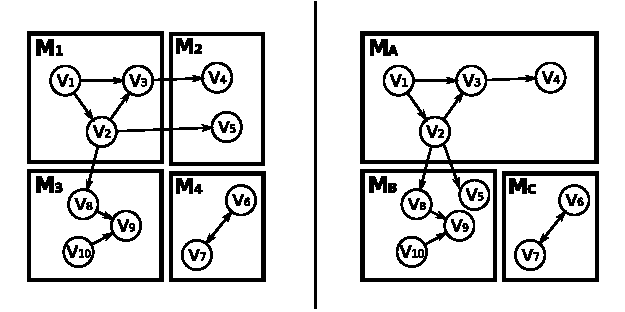
\includegraphics[scale=1]{figuras/redes-dupla}
	\caption{Dois agrupamentos de um mesmo sistema de software hipotético, descrito como um grafo que representa dependências entre classes.}
	\label{fig:mojo}
\end{figure}

% É fácil verificar se dois agrupamentos de um mesmo conjunto de entidades são idênticos ou não. Para comparar diferentes agrupamentos produzidos por algoritmos, no entanto, é preciso definir uma métrica de similaridade entre agrupamentos que seja capaz de determinar qual agrupamento de uma coleção de agrupamentos é mais similar a um agrupamento de referência.

No domínio de agrupamento de software, a métrica MoJo \cite{Tzerpos1999} tem sido bastante utilizada para medir a similaridade entre dois agrupamentos. A ideia por trás da métrica é que um agrupamento dado é muito similar a um agrupamento de referência se é possível transformar o primeiro agrupamento no segundo usando poucas operações do tipo mover e mesclar. A operação mover consiste de mover uma entidade de um módulo para outro módulo distinto. A operação mesclar consiste de mesclar dois módulos. O MoJo entre  dois agrupamentos é igual ao número de operações de mover e mesclar que são necessárias para transformar o primeiro agrupamento no segundo. Quanto menor o MoJo, maior a similaridade entre dois agrupamentos; agrupamentos idênticos têm MoJo igual a zero.

% A métrica MoJo não é simétrica. Para chegar a essa conclusão, basta observar que há uma operação de mesclar módulos, mas não uma operação de dividir um módulo em dois. No contexto de avaliação de algoritmos de agrupamento de software, é considerado o número de operações necessárias para transformar o agrupamento encontrado por um algoritmo no agrupamento de referência, e não o contrário.

Na Figura \ref{fig:mojo}, considerando que o agrupamento de referência é o segundo (o da direita), o MoJo entre os dois agrupamentos vale 2. Para transformar o primeiro agrupamento no segundo são necessárias, portanto, duas operações: mesclar os módulos $M_1$ e $M_2$, e mover o vértice $v_5$ para o módulo $M_3$. Após a realização dessas operações, os agrupamentos se tornam idênticos, considerando as correspondências $(M_1 \cup M_2) = M_A$, $M_3 = M_B$ e $M_4 = M_C$.

Observando que o valor MoJo entre dois agrupamentos com o mesmo número de entidades varia entre 0 e o número de entidades em cada agrupamento, $n$, é possível definir uma métrica, chamada MoJoSim, que mapeia o valor MoJo em uma escala de 0 a 1 \cite{Bittencourt2009}. O valor 0 representa a menor similaridade e o valor 1, a maior similaridade. O valor de MoJoSim entre dois agrupamentos é definido de acordo com a seguinte equação:

$$
\mathrm{MoJoSim}(X, Y) ~=~ 1 - \frac{\mathrm{MoJo}(X, Y)}{n}
$$

% Anquetil avaliou 

Wu, Hassan e Holt \cite{Wu2005} avaliaram os algoritmos Bunch, ACDC e algoritmos aglomerativos comparando, através da métrica MoJo, os agrupamentos encontrados pelos algoritmos com agrupamentos de referência de 5 sistemas de software em C e C++, representados como um grafo dos arquivos fonte e dependências estáticas entre os arquivos. Os agrupamentos de referência foram obtidos automaticamente a partir de uma análise da estrutura de diretórios dos sistemas. Cada diretório contendo pelo menos 5 arquivos fonte foi considerado um módulo do sistema. Bittencourt e Guerrero \cite{Bittencourt2009} realizaram um experimento semelhante, porém avaliando algoritmos de agrupamento estudados em outros domínios aplicados sobre um conjunto de 4 sistemas em Java.

\end{section}


% \begin{section}{Agrupamento}
% 
% A atividade de agrupamento consiste de agrupar um conjunto de entidades em subconjuntos, denominados módulos, de forma que, sob algum critério, as entidades agrupadas em um mesmo módulo possuem grande similaridade entre si e pequena similaridade com entidades que estão em outros módulos. Em muitas aplicações, a noção de módulo não é bem definida. Ainda assim, o agrupamento dos dados pode evidenciar relacionamentos existentes entre entidades e servir como ponto de partida de atividades como, por exemplo, a atribuição de arquivos de código-fonte a programadores.
% 
% O termo agrupamento designa tanto a atividade de agrupamento como o resultado dessa atividade, que é a organização das entidades analisadas em módulos. Existem diversos tipos de agrupamento:
% 
% \begin{itemize}
% 	\item hierárquico vs. partitivo: no agrupamento hierárquico, os módulos são sucessivamente agrupados em módulos de módulos. No agrupamento partitivo, apenas as entidades estão agrupadas em módulos. Uma organização hierárquica pode ser transformada em plana se a árvore da hierarquia for cortada em algum nível.
% 
% 	\item completo vs. parcial: na organização completa, todas as entidades pertencem a algum módulo; na organização parcial podem existir entidades sem módulos.
% 
% 	\item módulos sobrepostos vs. mutuamente exclusivos: na organização com módulos sobrepostos, podem existir entidades que pertencem a mais de um módulo; na organização de módulos mutuamente exclusivos, cada entidade pertence a no máximo um módulo.
% \end{itemize}
% 
% %%%%%%%% SIMILARIDADE
% 
% Para realizar o agrupamento de um conjunto de entidades de maneira sistemática, as seguintes questões devem ser consideradas:
% 
% \begin{itemize}
% 	\item identificação das entidades;
% 	\item a descrição das entidades;
% 	\item o algoritmo de agrupamento;
% \end{itemize}
% 
% A descrição das entidades determina as características a se considerar para determinar se duas entidades são mais ou menos similares. Por exemplo, se o objetivo é agrupar funções em um programa procedimental, as entidades são funções e as seguintes descrições, entre outras, podem ser adotadas para cada entidade:
% 
% \begin{itemize}
% 	\item conjunto das palavras usadas nos comentários que descrevem a função;
% 	\item conjunto dos programadores que trabalharam na função;
% 	\item conjunto das funções chamadas pela função;
% 	\item conjunto das variáveis manipuladas na função.
% \end{itemize}
% 
% As duas últimas descrições são chamadas de descrições formais, pois elas têm impacto sobre o comportamento do programa \cite{Anquetil1999}. As duas primeiras são descrições não-formais. 
% 
% Algoritmos de agrupamento são estudados em áreas diversas como a mineração de dados, a física estatística, a inteligência artificial e a engenharia de software. Alguns algoritmos são genéricos e dependem apenas de um conjunto de entidades e de uma função que define a similaridade entre entidades. Outros algoritmos são específicos para grafos.
% 
% \end{section}
% 
% \begin{section}{XXX}
% 
% Muitas abordagens de recuperação de arquitetura são baseadas na análise de código-fonte \cite{Pollet2007}. Uma parte destas abordagens usa algoritmos de clustering para determinar um agrupamento das entidades do código-fonte. Nesses trabalhos, as entidades podem ser funções e variáveis em sistema procedimentais CITE, tipos abstratos de dados CITE, arquivos-fonte CITE, classes em um sistema orientado a objetos CITE etc. Em outra dimensão, vários descrições são usadas para as entidades: nomes de identificadores CITE, co-mudança em sistemas de controle de versão CITE, co-uso em tempo de execução CITE, dependências estáticas no código-fonte etc.
% 
% Neste trabalho, optamos por estudar sistemas orientados a objetos escritos em Java, uma escolha que se justifica pela popularidade da linguagem de programação Java e do paradigma de programação orientada a objetos. Os sistemas são representados como conjuntos de classes, e cada classe é descrita através do conjunto de classes às quais ela faz referência em seu código-fonte. Desta forma, os sistemas de software podem ser representados como grafos orientados. Essa representação de um sistema de software será chamada, daqui em diante, de \emph{rede de software}.
% 
% % Vale ressaltar que referências estáticas no código-fonte são uma aproximação para o conceito de dependência. Diz-se que uma classe, A, depende de outra classe, B, quando o funcionamento correto da classe A depende de uma implementação correta da classe B (Parnas - Designing software for ease of extension and contraction). 
% 	
% \end{section}
% 
% 
% % As descrições mais usadas em pesquisa são as descrições formais.
% % 
% % As descrições das entidades são usadas como base de métricas de similaridade. Considerando o exemplo em que as entidades são funções e a descrição de uma função é o conjunto de funções por ela chamadas, consideremos X e Y duas descrições de funções. A similaridade de Jaccard entre as duas entidades, sim($X, Y$), é dada por:
% % 
% % $$
% % \mathrm{sim}(X, Y) ~=~ \frac{X \cap Y}{X \cup Y}
% % $$
% % 
% % A métrica de similaridade de Jaccard é comumente usada em estudos de agrupamento no domínio de sistemas de software \cite{Anquetil1999,Wu2005}, e por isso será usada também neste estudo.
% % 
% % 
% % %%%%%%%%%%%% ALGORITMO
% % 
% % Para este estudo, foram selecionados 4 algoritmos de agrupamento: 
% % 
% % \begin{itemize}
% % 	\item algoritmo hierárquico aglomerativo (AHA): é um algoritmo de propósito geral que produz agrupamentos hierárquicos.
% % 	\item Bunch: é um algoritmo que opera sobre grafos orientados e foi proposto especificamente para o domínio de software.
% % 	\item ACDC: da mesma forma que o Bunch, opera sobre grafos orientados e foi proposto para o domínio de software.
% % 	\item Infomap: opera sobre grafos orientados e foi proposto para o problema de detectar comunidades em redes sociais.
% % \end{itemize}
% % 
% % % XXX Falar brevemente sobre o funcionamento de cada algoritmo.
% % 
% % 
% % 
% % % Agrupamento é um problema antigo. Taxonomia etc.
% % % Representação de dados
% % 
% % % Que representação usar para software? Grafo: sólidas fundações teóricas, existem algoritmos de agrupamento especificamente projetados para grafos.
% % % em particular, grafos orientados
% % % extração usando análise estática, por ser de aplicação mais geral. Tipos de dependências.
% % 
% % \begin{section}{Introdução}
% % 	
% % \end{section}
% % 
% % % INTRODUÇÃO COM UM APANHADO DO QUE VIRÁ
% % % --
% % % TEORIA DOS GRAFOS. orientado/ponderado
% % % GRAFOS ORGANIZADOS EM MÓDULOS - mencionar que existem algoritmos de agrupamento
% % % VALIDAÇÃO DE ORGANIZAÇÃO EM MÓDULOS - interna, externa...
% % % EXTRAÇÃO DE GRAFOS A PARTIR DE SOFTWARE - análise estática/dinâmica...
% % % AGRUPAMENTO DE SOFTWARE - identificadores, co-mudanças...
% % 
% % Grafo é uma representação matemática de um conjunto de entidades na qual duas entidades podem ou não estar relacionadas. Em um grafo, as entidades são chamadas vértices e as relações entre vértices são chamadas arestas. Grafos são definidos de acordo com as seguintes dimensões:
% % 
% % - orientado vs. não-orientado. Nos grafos não-orientados, as arestas representam uma relação simétrica entre dois vértices. No caso dos grafos orientados, cada aresta possui um vértice de origem e um vértice de destino. Diz-se que $a$ é uma aresta de $v_1$ para $v_2$ quando $v_1$ é a origem e $v_2$ é o destino de $a$. Nos grafos orientados existem também arestas bidirecionais, que equivalem a duas arestas com orientações opostas.
% % 
% % - ponderado vs. não-ponderado. Em alguns casos, é atribuído um valor a cada aresta, denominado peso. Os pesos podem representar, por exemplo, a força da ligação entre dois vértices. Nos grafos não-ponderados não há pesos ou, equivalentemente, todas as arestas possuem o mesmo peso.
% % 
% % - grafos simples vs. multigrafos. Nos grafos simples, não podem existir duas arestas ligando o mesmo par de vértices, e nem autolaços --- arestas que ligam um vértice a ele próprio. Nos multigrafos cada par de vértices pode ser ligado por diversas arestas e os autolaços são permitidos.
% % 
% % No decorrer deste trabalho serão estudados grafos simples, orientados e não-ponderados. % XXX falar agora ou deixar pra mais tarde?
% % 
% % \begin{section}{Organização em módulos}
% % 
% % Um conceito importante no estudo de algoritmos de agrupamento é o conceito de organização em módulos. 
% % para simplificar, vamos chamar de particionamento...
% % 
% % \end{section}
% % 
% % \begin{section}{Algoritmos de agrupamento}
% % 
% % Algoritmos de agrupamento têm por objetivo agrupar entidades em subconjuntos, denominados módulos, de forma, sob algum critério, as entidades agrupadas em um módulo possuem grande similaridade entre si e pequena similaridade com vértices de outros módulos. Após a aplicação de um algoritmo de agrupamento sobre um conjunto de entidades, diz-se que as entidades estão organizadas em módulos.
% % 
% % % Exemplo: entidades = pontos no plano. dois pontos são colocados no mesmo grupo se a distância euclideana entre eles é menor do que ``d''.
% % 
% % Uma organização em módulos pode ser classificada de diversas maneiras:
% % 
% % hierárquico vs. partitivo: na organização hierárquica, os módulos são sucessivamente agrupados em módulos de módulos. Na plana, apenas as entidades estão agrupadas em módulos. Uma organização hierárquica pode ser transformada em plana se a árvore da hierarquia for cortada em algum nível.
% % 
% % completo vs. parcial: na organização completa, todas as entidades pertencem a algum módulo; na organização parcial podem existir entidades sem módulos.
% % 
% % módulos sobrepostos vs. mutuamente exclusivos: na organização com módulos sobrepostos, podem existir entidades que pertencem a mais de um módulo; na organização de módulos mutuamente exclusivos, cada entidade pertence a no máximo um módulo.
% % 
% % %% NESTE trabalho estudamos apenas algoritmos que produzem organizações completas e com módulos mutuamente exclusivos. (a fim de facilitar a comparação das organizações em módulos).
% % 
% % No estudo de redes sociais, algoritmos de agrupamento que operam sobre redes, agrupando seus vértices, são chamados de algoritmos de detecção de comunidades.
% % 
% % Na física, detecção de comunidades.
% % 
% % Critérios: validade interna, validade externa etc.
% % 
% % \end{section}
% % \begin{section}{Agrupamento de software}
% % 
% % De um ponto de vista amplo, agrupa artefatos de software de um sistema computacional. Código-fonte, UML, documentação...
% % 
% % Uma vertente, estudada neste trabalho, é o agrupamento de entidades do código-fonte. O próprio conceito de entidade não é bem definido. Podem ser funções e variáveis em sistema procedimentais CITE, tipos abstratos de dados CITE, arquivos-fonte CITE, classes em um sistema orientado a objetos CITE etc.
% % 
% % Há vários critérios: nomes de identificadores CITE, co-mudança em sistemas de controle de versão CITE, co-uso em tempo de execução CITE, relações estáticas no código-fonte etc.
% % 
% % Neste trabalho estudaremos relações estáticas em programas orientados a objetos. Ainda assim, um software pode ser representado de diversas formas.
% % 
% % \end{section}
% % \begin{section}{Grafo de dependências entre entidades}
% % 
% % Grafo orientado não-ponderado.
% % Entidades: classes e interfaces Java.
% % 
% % Significado de ``dependência''.
% % 
% % Limitações da análise estática.
% % 
% % Ferramenta DependencyFinder.
% % 
% % Dependências:
% %   classe é subclasse de classe
% %   classe implementa interface
% %   classe chama método de classe
% %   classe acessa atributo de classe
% %   ...
% % 
% % \end{section}
% % \begin{section}{Algoritmos de agrupamento usados em software e selecionados para este trabalho}
% % 
% % Hierárquico (mineração de dados), usado por Anquetil, Wu etc.
% % 
% % ACDC (ES)
% % 
% % Bunch (ES)
% % 
% % Infomap (física estatística, detecção de comunidades), estudado por Lancichinetti.
% % 
% % \end{section}
% 
% % Avaliação de agrupamento de software deve ser uma seção separada ou parte da introdução e da seção de agrupamento em mineração de dados?
% 
